% !TeX spellcheck = ru_RU
\documentclass[10pt,a4paper,openany]{book}
\usepackage[russian]{babel}
\usepackage[utf8]{inputenc}
\usepackage{indentfirst}
\usepackage{amsthm}
\usepackage{amsmath}
\usepackage{tabularx,ragged2e,booktabs}
\usepackage{tikz}
\usepackage{epstopdf}
\usepackage{graphicx}
\usepackage[style=russian]{csquotes}
\usepackage{multirow}
\usepackage{url}
\usepackage{hyperref}

\begin{document}
\title{Компьютерные сети \\ Учебное пособие}
\date{}
\maketitle

\theoremstyle{definition}
\newtheorem{exmp}{Пример}[section]

\usetikzlibrary{arrows,positioning} 
\tikzset{
	%Define standard arrow tip
	>=stealth',
}

\tableofcontents
\chapter*{Предисловие}
\input{intro}
\chapter{Введение в компьютерные сети}
% !TeX spellcheck = ru_RU
\section{Эталонные модели сетевого взаимодействия}
Существуют две основные модели, описывающие взаимодействие устройств в компьютерных сетях.
\begin{itemize}
	\item OSI (содержит 7 уровней)
	\item TCP/IP (содержит 4 уровней)
\end{itemize}
\begin{table}[h!]
	\centering
	\begin{tabular}{|l|l|l|l|}
		\hline
			\multicolumn{2}{|c|}{Уровень} & \multicolumn{1}{c|}{Функции} & \multicolumn{1}{c|}{Примеры протоколов} \\ \hline
			7 & Приложения & Протоколы пользовательских приложений & HTTP(S), POP3, SMTP \\ \hline
			6 & Представления & Сжимание, шифрование &  \\ \hline
			5 & Сессионный & Контроль сессии &  \\ \hline
			4 & Транспортный &  & UDP, TCP \\ \hline
			3 & Сетевой & Протоколы глобального взаимодействия & IPv4, IPv6 \\ \hline
			2 & Канальный & Протоколы локального взаимодействия & Ethernet (MAC) \\ \hline
			1 & Физический & Кабели, коннекторы & Ethernet (PHY) \\ \hline
	\end{tabular}
	\caption{Структура модели OSI}
	\label{tbl:osi}
\end{table}
Структура первой модели представлена в таблице~\ref{tbl:osi} вместе с примерами протоколов, работающих на разных уровнях. Все сетевые устройства работают на различных уровнях (стоит отметить, что существуют устройства, затрагивающие сразу несколько уровней). Вот несколько примеров:
\begin{itemize}
	\item физический --- концентраторы, повторители, медиаконвертеры;
	\item канальный --- мосты, коммутаторы
	\item сетевой --- маршрутизаторы (роутеры)
	\item транспортный --- шлюзы и брандмауэры
\end{itemize}
Некоторые из этих устройств будут подробно рассмотрены позже.
\section{Инкапсуляция и декапсуляция}
\begin{figure}[h!]
	\centering
	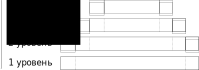
\includegraphics[width=0.8\linewidth]{pic/incapsulation.pdf}
	\caption{Процесс инкапсуляции}
	\label{fig:incapsulation}
\end{figure}
Рассмотрим подробнее схему передачи данных в компьютерных сетях. (см. рис.~\ref{fig:incapsulation}). Когда на уровень приложений поступают данные для передачи, протокол 7 уровня добавляет к данным какой-то свой заголовок и концевик (необязательно) и передает полученный блок данных на уровень ниже. Далее процесс повторяется, пока пакет не дойдет до физического уровня, когда, собственно, начнется передача данных. Во время приема данных происходит обратный процесс --- декапсуляция. 

Важно конкретно называть блоки данных (Protocol Data Unit, PDU), которыми оперируют разные уровни модели OSI. Так, в частности:
\begin{itemize}
	\item 1 уровень --- бит;
	\item 2 уровень --- кадр;
	\item 3 уровень --- пакет;
	\item 4 уровень --- сегмент.
\end{itemize}

Стоит отметить, что каждое устройство производит инкапсуляцию и декапсуляцию лишь до того уровня на котором оно работает (см. рис~\ref{fig:incapsulation_devices}).
\begin{figure}[h!]
	\centering
	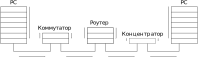
\includegraphics[width=0.8\linewidth]{pic/incapsulation_devices.pdf}
	\caption{Инкапсуляция и декапсуляция на различных устройствах}
	\label{fig:incapsulation_devices}
\end{figure}

\section{Литература}
\begin{itemize}
	\item ICND1 \cite{icnd1eng}, Глава 1.
\end{itemize}
\chapter{Ethernet}
% !TeX spellcheck = ru_RU
\section{Канальный уровень}
\subsection{Структура кадра}
Блоки, в которых передаются данные в Ethernet, называются кадрами или фреймами (англ. frame). Их структура изображена в таблице~\ref{tbl:ethernet_frame_structure}. Рассмотрим функции всех полей в кадре более подробно. 
\begin{table}[h!]
	\centering
	\begin{tabular}{|c|c|c|c|c|}
		\hline
		\begin{tabular}[c]{@{}c@{}}DAddr\\ 6 байт\end{tabular} & \begin{tabular}[c]{@{}c@{}}SAddr\\ 6 байт\end{tabular} & \begin{tabular}[c]{@{}c@{}}EtherType\\ 2 байта\end{tabular} & \begin{tabular}[c]{@{}c@{}}Data\\ 46-1500 байт\end{tabular} & \begin{tabular}[c]{@{}c@{}}FCS\\ 4 байта\end{tabular} \\ \hline
	\end{tabular}
	\caption{Структура кадра Ethernet}
	\label{tbl:ethernet_frame_structure}
\end{table}
\begin{itemize}
	\item $DAddr$ и $SAddr$ --- это адреса получателя и отправителя. Каждое устройство получает при выпуске свой уникальный MAC-адрес, состоящий из 6 байт (см. рис~\ref{fig:mac_address_structure}). Первые три байта содержат уникальный идентификатор компании-производителя, которая сама назначает значения последних трёх байтов каждому своему устройству. Стоит отметить, что каждый производитель может иметь несколько уникальных идентификаторов. 
	\item Поле $EtherType$ необходимо для определения того, данные какого протокола более высокого уровня лежат внутри кадра.
	\item $Data$ содержит непосредственно сами передаваемые данные (например, пакет IP).
	\item $FCS$ --- это контрольная сумма. Она необходима для определения наличия ошибок, возникших при передаче кадра.
\end{itemize}

Также в самом начале фрейма находится преамбула, которая используется для синхронизации двух устройств между собой.

Длина кадров меняется в пределах от 64 до 1518 байт. Ограничение сверху нужно для того, чтобы устройство не занимало канал на слишком большой промежуток времени, в то время как ограничение снизу необходимо для возможности определения коллизий (т.е. попыток одновременной передачи данных двумя устройствами). Если кадр будет слишком коротким, устройство не успеет задетектировать наличие передачи от другого устройства из-за конечной скорости распространения сигналов в среде. Устройство детектирует коллизии путем сравнения передаваемого сигнала с сигналом, реально наблюдаемым в среде. При коллизии передаваемые сигналы с двух устройств наложатся друг на друга, и наблюдаемый сигнал на каждом устройстве будет отличаться от передаваемого.
\begin{figure}[t!]
	\centering
	\begin{tabular}{cc}
		\hline
		\multicolumn{1}{|c|}{3 байта} & \multicolumn{1}{c|}{3 байта} \\ \hline
		идентификатор производителя & идентификатор устройства
	\end{tabular}
	\caption{Структура MAC-адреса}
	\label{fig:mac_address_structure}
\end{figure}
\subsection{Виды MAC-адресов}
Существует три вида MAC-адресов:
\begin{itemize}
	\item unicast адреса, предназначенные для передачи одному одному устройству;
	\item broadcast адреса, используемые для широковещательной рассылки;
	\item multicast адреса, используемые для передачи нескольким устройствам.
\end{itemize}

Широковещательная рассылка означает, что фрейм предназначается всем устройствам в сегменте. Широковещательный адрес всего один -- $FF:FF:FF:FF:FF:FF$. 

В данном курсе multicast адреса особо рассматриваться не будут. Однако стоит отметить, что если младший бит первого байта MAC-адреса установлен в 1, то мы имеем дело с multicast адресом. 
\subsection{Методы доступа к каналу}
Для доступа к каналу (среде передачи данных) в Ethernet используется CSMA/CD (англ. Carrier Sense Multiple Access with Collision Detection — множественный доступ с прослушиванием несущей и обнаружением коллизий). Суть этого метода заключается в следующем.

При неудачной попытке передачи устройство выжидает случайный период времени, равномерно распределенный на интервале $[1, 2^n-1] \cdot T$, где $T$ --- время передачи 512 бит, а $n$ --- номер попытки отправки фрейма. Чтобы время ожидания начала передачи не было слишком большим, максимальное количество неудачный попыток ограничено четырьмя. 

Очевидно, что с ростом количества активных узлов в сегменте работоспособность у данной схемы сильно проседает.

\subsection{Литература}
\begin{itemize}
	\item ICND1 \cite{icnd1eng}, Глава 2;
	\item Олифер \cite{olipher}, Глава 12, с. 360-372.
\end{itemize}
% !TeX spellcheck = ru_RU
\section{Физический уровень}
\subsection{Повторители}
Из-за наличия затухания в среде существуют ограничения на длину используемых кабелей. Для построения сильно распределенных сетей можно использовать устройства, называемые повторителями или репитерами. Они усиливают и очищают сигнал, при этом не зная ничего о самом передаваемом фрейме, т.е. работая только с электрическим сигналом. Отсюда следует, что повторители работают на физическом уровне модели OSI.
\begin{figure}[ht!]
	\centering
	\begin{tikzpicture}
		\draw (-4, 0) -- (0,0);
		\draw (0, 0) -- (4,0);
		
		\draw (-3, 0) -- (-3, 1);
		\node at (-3, 1) [label=above:A] {\includegraphics{pic/pc.eps}};
		
		\draw (-2, -1) -- (-2, 0);
		\node at (-2, -1) [label=below:B] {\includegraphics{pic/pc.eps}};
		
		\draw (3, 0) -- (3, 1);
		\node at (3, 1) [label=above:D] {\includegraphics{pic/pc.eps}};
		
		\draw (2, -1) -- (2, 0);
		\node at (2, -1) [label=below:C] {\includegraphics{pic/pc.eps}};
		
		\draw[->] (-3.9, 1.5) -- (-3.9, 0.45);
		\draw[->] (-2.9, -1.5) -- (-2.9, -0.45);
		
		\draw[->] (-4, -0.6) -- (-2.5, 0);
		
		\node at (-4, -0.5) [below] {Коллизия};
		
		\node at (0, 0) [label=above:Повторитель] {\includegraphics{pic/repeater.eps}};
	\end{tikzpicture}
	\caption{Пример применения повторителя}
	\label{fig:repeater}
\end{figure}

Обратимся к рис.~\ref{fig:repeater}. Пусть узлы A и B решили одновременно начать передачу данных и попали в коллизию. Установка повторителя никак на нее влияет, и он просто передаст коллизию во всю сеть. 
\subsection{Концентраторы}
С течением времени на место репитеров пришли концентраторы (хабы). Логика их работы аналогична повторителям, однако полученный сигнал распространяется не через один порт, а через все порты хаба (кроме того, через который сигнал был получен). Использование хабов позволяет значительно увеличить размеры сетевых сегментов. 
\begin{figure}[h!]
	\centering
	\begin{tikzpicture}
		\draw (-4, 0) -- (0,0);
		\draw (0, 0) -- (4,0);
		\draw (0, 0) -- (0, -3);
		
		\draw (-3, 0) -- (-3, 1);
		\node at (-3, 1) [label=above:A] {\includegraphics{pic/pc.eps}};
		
		\draw (-2.25, -1) -- (-2.25, 0);
		\node at (-2.25, -1) [label=below:B] {\includegraphics{pic/pc.eps}};
		
		\draw (-1.5, 0) -- (-1.5, 1);
		\node at (-1.5, 1) [label=above:C] {\includegraphics{pic/pc.eps}};
		
		\draw (3, 0) -- (3, 1);
		\node at (3, 1) [label=above:E] {\includegraphics{pic/pc.eps}};
		
		\draw (2, -1) -- (2, 0);
		\node at (2, -1) [label=below:D] {\includegraphics{pic/pc.eps}};
		
		\draw (0, -2) -- (-1, -2);
		\node at (-1, -2) [label=below:F] {\includegraphics{pic/pc.eps}};
		
		\node at (0, 0) [label=above:Хаб] {\includegraphics{pic/hub.eps}};
	\end{tikzpicture}
	\caption{Пример применения хаба}
	\label{fig:hub}
\end{figure}

Однако концентраторы обладают рядом существенных недостатков. Обратимся к рис.~\ref{fig:hub}. Фрейм, отправленный от A к С, получат все устройства, но, так как MAC-адрес получателя относится только к C, то все остальные должны просто отбросить полученный кадр (но это только в теории!), то есть фрейм будет получен всеми сетевыми устройствами независимо от того, кому он был предназначен. Также, аналогично повторителям, хабы никак не защищают от коллизий.
\subsection{Симплекс, полудуплекс и дуплекс}
Существует три способа передачи данных между двумя устройствами:
\begin{itemize}
	\item симплексный --- передача данных возможна лишь в одну сторону;
	\item полудуплексный --- одновременная передача данных возможна лишь в одном направлении;
	\item полнодуплексный (англ. full-duplex) --- одновременная передача данных возможна в обоих направлениях.
\end{itemize}
Сети, построенные на основе топологии \enquote{Шина}, всегда используют полудуплексную передачу. Стоит отметить, что при использовании полнодуплексного способа связи коллизии невозможны в принципе.
\subsection{Литература}
\begin{itemize}
	\item ICND1 \cite{icnd1eng}, Глава 2.
\end{itemize}
\chapter{Коммутация}
% !TeX spellcheck = ru_RU
\section{Устройства 2 уровня модели OSI}
\subsection{Широковещательные и коллизионные домены}
\textbf{Широковещательный домен} - часть сети, в которой широковещательнный фрейм, посланный с любого устройства, достигнет всех остальных устройств в данном домене.
\textbf{Коллизионный домен} - часть сети, в которой между двумя устройствами может произойти коллизия.
\subsection{Мосты и мостовые таблицы}
Мосты, также как и повторители, предназначены для связи двух сегментов Ethernet между собой. Однако, логика работы этих устройств сильно отличается.

\begin{table}[h!]
	\centering
	\begin{tabular}{|c|c|c|}
		\hline
		Порт & MAC & Время \\ \hline
		1 & $MAC_a$ & $t_1$ \\ \hline
		1 & $MAC_b$ & $t_2$ \\ \hline
		1 & $MAC_c$ & $t_3$ \\ \hline
		2 & $MAC_d$ & $t_4$ \\ \hline
		\multicolumn{3}{|c|}{...} \\ \hline
	\end{tabular}
	\caption{Пример мостовой таблицы}
	\label{tbl:cam_table}
\end{table}
Каждый мост строит MAC/CAM/мостовую таблицу. Эта таблица предназначена для оптимизации передачи фрейма. Ее структура показана в табл.~\ref{tbl:cam_table}. В поле $Port$ содержится номер порта, с которого был получен фрейм с MAC-адресом, указанным в поле $MAC$. Таблица может заполняться как автоматически самим мостом, так и администратором. На размер мостовой таблицы имеются ограничения: от 8000 записей в простых устройствах до 128000 в более дорогих.

\begin{figure}[h!]
	\centering
	\begin{tikzpicture}
		\draw (-4.5, 0) -- (0,0);
		\draw (0, 0) -- (4.5,0);
		
		\draw (-4, 0) -- (-4, 1);
		\node at (-4, 1) [label=above:A] {\includegraphics{pic/pc.eps}};
		
		\draw (-3, -1) -- (-3, 0);
		\node at (-3, -1) [label=below:B] {\includegraphics{pic/pc.eps}};
		
		\draw (-2, 0) -- (-2, 1);
		\node at (-2, 1) [label=above:C] {\includegraphics{pic/pc.eps}};
		
		\draw (4, 0) -- (4, 1);
		\node at (4, 1) [label=above:F] {\includegraphics{pic/pc.eps}};
		
		\draw (3, -1) -- (3, 0);
		\node at (3, -1) [label=below:E] {\includegraphics{pic/pc.eps}};
		
		\draw (2, 0) -- (2, 1);
		\node at (2, 1) [label=above:D] {\includegraphics{pic/pc.eps}};
		
		\draw[->] (-4.9, 1.5) -- (-4.9, 0.45);
		\draw[<-] (-3.9, -1.5) -- (-3.9, -0.45);
		\draw[<-] (-2.9, 1.5) -- (-2.9, 0.45);
		\draw[->] (-1.9, -0.3) -- (-0.8, -0.3);
		
		\node at (0, 0) [label=above:Мост] {\includegraphics{pic/bridge.eps}};
		\node at (-0.6, 0.1) [above left] {1};
		\node at (0.7, 0.1) [above right] {2};
	\end{tikzpicture}
	\caption{Пример применения моста}
	\label{fig:bridge}
\end{figure}
Рассмотрим принцип работы моста на примере (см. рис.~\ref{fig:bridge}). 
\begin{itemize}
	\item Пусть узел A посылает фрейм узлу B. В этом случае мост видит, что A и B в одном сегменте, и игнорирует данный фрейм, так как узел B уже получил его. 
	\item Если узел А пошлёт фрейм узлу D, то мост передаст фрейм в тот сегмент, где находится узел D. Если A и D начнут передачу данных одновременно, то коллизии не произойдет. При коллизиях мост ведет себя так же, как и обычный узел с удержанием фрейма в буфере неопределённое время.
	\item Если узел C переедет в тот сегмент, где находится D, то через некоторое время мост пометит его запись в таблице как устаревшую и удалит ее из таблицы. Аналогичная ситуация произойдёт, если узел просто выключится.
	\item Широковещательные фреймы передаются мостом также и в другой сегмент сети.
	\item Если на мост придёт фрейм для неизвестного получателя, то он обработается как широковещательный.
\end{itemize}

Когда таблица заполнена и в сети появляется новое устройство, то поведение моста будет зависеть от архитектуры конкретного устройства: либо будут удаляться старые записи (даже если время не истекло), либо новые записи не будут добавлены.
\subsection{Коммутаторы}
Коммутатор (свитч) --- это по своей сути многопортовый мост. Именно эти устройства составляет основу современных локальный сетей Ethernet. 
\begin{figure}[h!]
	\centering
	\begin{tikzpicture}
		\draw (-4, 0) -- (0,0);
		\draw (0, 0) -- (4,0);
		\draw (0, 0) -- (0, -3);
		
		\draw (-3, 0) -- (-3, 1);
		\node at (-3, 1) [label=above:A] {\includegraphics{pic/pc.eps}};
		
		\draw (-2.25, -1) -- (-2.25, 0);
		\node at (-2.25, -1) [label=below:B] {\includegraphics{pic/pc.eps}};
		
		\draw (3, 0) -- (3, 1);
		\node at (3, 1) [label=above:E] {\includegraphics{pic/pc.eps}};
		
		\draw (2, -1) -- (2, 0);
		\node at (2, -1) [label=below:D] {\includegraphics{pic/pc.eps}};
		
		\draw (0, -2) -- (-1, -2);
		\node at (-1, -2) [label=below:C] {\includegraphics{pic/pc.eps}};
		
		\node at (0, 0) [label=above:Коммутатор] {\includegraphics{pic/switch.eps}};
	\end{tikzpicture}
	\caption{Коммутатор}
	\label{fig:switch}
\end{figure}

С внедрением коммутаторов проблемы в сетях стали возникать только в пределах одного сегмента, поэтому количество устройств, подключенных в одном сегменте, стали уменьшать. Если к каждому сегменту подключить лишь один узел и использовать полный дуплекс, то коллизий в такой сети попросту \textbf{не будет}.

Также, как и в мостах, в коммутаторах есть буферы, в которых еще не отправленные фреймы хранятся некоторое время. Благодаря этому коммутаторы, в отличие от концентратора, позволяют подключать разноскоростное оборудование.

\begin{figure}[h!]
	\centering
	\begin{minipage}[h]{0.45\linewidth}
		\center {
			\begin{tabular}{|c|c|c|}
				\hline
				Порт & MAC & Время \\ \hline
				1 & $A$ & $t_1$ \\ \hline
				2 & $B$ & $t_2$ \\ \hline
				3 & $C$ & $t_3$ \\ \hline
			\end{tabular}
		}
	\end{minipage}
	\hfill
	\begin{minipage}[h]{0.45\linewidth}
		\center {
			\begin{tikzpicture}
					\draw (-2, -2) -- (0,0);
					\draw (0, -2) -- (0,0);
					\draw (2, -2) -- (0,0);
			
					\node at (-2, -2) [label=below:A] {\includegraphics{pic/pc.eps}};
					\node at (0, -2) [label=below:B] {\includegraphics{pic/pc.eps}};
					\node at (2, -2) [label=below:C] {\includegraphics{pic/pc.eps}};
			
					\node at (0, 0) {\includegraphics{pic/switch.eps}};
					\node at (-0.65, -0.35) [below left] {1};
					\node at (0, -0.4) [below left] {2};
					\node at (0.65, -0.35) [below right] {3};
			\end{tikzpicture}
		}
	\end{minipage}
	\hfill
	\vfill
	\caption{Пример, иллюстрирующий проблемы безопасности}
	\label{fig:switch_security}
\end{figure}
Использование коммутаторов также порождает некоторые проблемы, связанные с безопасностью. Рассмотрим следующий пример (см. рис.~\ref{fig:switch_security}). Если узел C подменит свой MAC-адрес с C на B, то фреймы, предназначенные узлу B, будут приходить узлу C до тех пор, пока узел B не обновит запись в мостовой таблице своим фреймом с правильным MAC-адресом.
\section{Режимы коммутации сетей}
Существует три режима коммутации сетей:
\begin{itemize}
	\item \textbf{store and forward} (фрейм копируется в буфер целиком, и только после этого начинается обработка: проверка контрольной суммы, а затем уже работа с мостовой таблицей);
	\item \textbf{cut-through} (коммутатор получает первые 6 байт от начального заголовка фрейма (т.е. MAC-адрес получателя) и сразу проверяет мостовую таблицу и отправляет фрейм);
	\item \textbf{fragment-free} (коммутатор принимает первые 64 байт и затем работает как cut-through, однако, в отличие от последнего, этот режим спасает от фреймов, поврежденных во время коллизий).
\end{itemize}

\section{Литература}
\begin{itemize}
	\item ICND1 \cite{icnd1eng}, Глава 6;
	\item Олифер \cite{olipher}, Глава 13.
\end{itemize}
% !TeX spellcheck = ru_RU
\section{Протокол STP}
\subsection{Литература}
\begin{itemize}
	\item Олифер \cite{olipher}, Глава 14, с. 449-459;
	\item ICND2 \cite{icnd2eng}, Глава 2.
\end{itemize}
\chapter{Протокол IPv4}
% !TeX spellcheck = ru_RU
\section{Версии протокола IP}
На данный момент существуют две версии протокола IP: 
\begin{itemize}
	\item IPv4, являющаяся наиболее используемой на данный момент
	\item IPv6, постепенно приходящая на замену IPv4
\end{itemize}

В данной главе рассматривается IPv4, IPv6 будет рассмотрен позднее.
\section{Адресация}
\subsection{IP-адреса}
В IPv4 используются четырехбайтовые адреса, например, $192.168.1.1$. Введение новых адресов в дополнение к MAC-адресам необходимо для создания иерархии в сетях. IP-адреса не привязаны к железу, и их можно группировать в подсети.
\subsection{Классовая адресация}
Ранее в IPv4 существовало 5 классов IP-адресов (см. табл.~\ref{tbl:ip_classes}). 
\begin{table}[h!]
	\centering
	\begin{tabular}{|c|l|l|}
		\hline
		Класс & \multicolumn{1}{c|}{Значения первого октета} & \multicolumn{1}{c|}{Тип} \\ \hline
		A & 1-126 & \multirow{3}{*}{unicast} \\ \cline{1-2}
		\textit{B} & 128-191 &  \\ \cline{1-2}
		C & 192-223 &  \\ \hline
		D & 224-239 & multicast \\ \hline
		E & 240-255 & экспериментальные \\ \hline
	\end{tabular}
	\caption{Классы IP-адресов}
	\label{tbl:ip_classes}
\end{table}

Помимо этого, выделяется особый широковещательный адрес $255.255.255.255$.

Классы были необходимы для введения группировки IP-адресов на подсети, позволяющей существенно уменьшить размеры таблиц маршрутизации.

\begin{figure}[h!]
	\centering
	\begin{tikzpicture}
		\draw (-4.8, 0) -- (-3.3, 0);
		\fill[black] (-3.2, 0) circle (1.25pt);
		\draw (-3.1, 0) -- (-1.6, 0);
		\fill[black] (-1.5, 0) circle (1.25pt);
		\draw (-1.4, 0) -- (0.1, 0);
		\fill[black] (0.2, 0) circle (1.25pt);
		\draw (0.3, 0) -- (1.8, 0);
		\draw[red] (0.2, 0.4) -- (0.2, -0.4);
		
		\node at (3.5, 0) [right] {Класс C};
		\node at (-2.35, 0) [below] {Сетевая часть};
		\node at (0.2, 0) [below right] {Хостовая часть};
		
		\draw (-4.8, -1) -- (-3.3, -1);
		\fill[black] (-3.2, -1) circle (1.25pt);
		\draw (-3.1, -1) -- (-1.6, -1);
		\fill[black] (-1.5, -1) circle (1.25pt);
		\draw (-1.4, -1) -- (0.1, -1);
		\fill[black] (0.2, -1) circle (1.25pt);
		\draw (0.3, -1) -- (1.8, -1);
		\draw[red] (-1.5, -0.6) -- (-1.5, -1.4);
		
		\node at (3.5, -1) [right] {Класс B};
		\node at (-3.2, -1) [below] {Сетевая часть};
		\node at (0.3, -1) [below] {Хостовая часть};
		
		\draw (-4.8, -2) -- (-3.3, -2);
		\fill[black] (-3.2, -2) circle (1.25pt);
		\draw (-3.1, -2) -- (-1.6, -2);
		\fill[black] (-1.5, -2) circle (1.25pt);
		\draw (-1.4, -2) -- (0.1, -2);
		\fill[black] (0.2, -2) circle (1.25pt);
		\draw (0.3, -2) -- (1.8, -2);
		\draw[red] (-3.2, -1.6) -- (-3.2, -2.4);
		
		\node at (3.5, -2) [right] {Класс A};
		\node at (-3.2, -2) [below left] {Сетевая часть};
		\node at (-0.65, -2) [below] {Хостовая часть};
	\end{tikzpicture}
	\caption{Сетевая и хостовая часть IP-адреса}
	\label{fig:ip_classes}
\end{figure}

Для этого вводится деление адреса на сетевую и хостовую часть( см. рис.~\ref{fig:ip_classes}). Адреса узлов, находящихся в одном сегменте сети, должны иметь одинаковые сетевые, но разные хостовые части.

\begin{exmp}
Рассмотрим два IP-адреса класса A: $\underline{\mathbf{10}}.10.1.1$ и $\underline{\mathbf{10}}.11.12.13$. Сетевая часть первого адреса равна сетевой части второго адреса, следовательно, они принадлежат одной подсети.
\end{exmp}

\subsection{Бесклассовая адресация}
Для определения того, принадлежат ли адреса одной подсети, в современных сетях используются маски подсети -- 32-битные числа. Маска подсети имеет строго фиксированный формат, имеющий следующий двоичный вид: $\underbrace{1111...0000}_\text{32 бита}$. Важно, что сначала идет несколько единиц, а затем только нули. Сетевая часть IP-адреса имеет 

\begin{exmp}
Рассмотрим адрес $1.2.3.4$ с маской $255.255.255.0$. Сетевая часть в этом случае будет определяться следующим образом:
\begin{table}[h!]
	\centering
	\begin{tabular}{|l|l|l|}
		\hline
		\multicolumn{1}{|l|}{} & \multicolumn{1}{c|}{Десятичный вид} & \multicolumn{1}{c|}{Двоичный вид}  \\ \hline
		IP-адрес & 1.2.3.4        & $\underbrace{0000001.00000010.00000011}_\text{Сетевая часть}.\underbrace{00000100}_\text{Хостовая}$ \\ \hline
		Маска    & 255.255.255.0  & 1111111.11111111.11111111.00000000 \\ \hline
	\end{tabular}
	\caption{Пример применения маски}
	\label{tbl:ip_maskexample}
\end{table}

Также можно использовать запись $1.2.3.4/24$, это эквивалентно применению маски $255.255.255.0$.
\end{exmp}

Стоит отметить, что маски позволяют проводить границу IP-адреса где угодно. 

\subsection{Количество хостов в подсети}
Стоит отметить, что внутри каждой подсети зарезервировано два адреса со следующими хостовыми частями:
\begin{itemize}
	\item $00...0$ -- адрес сети, не назначается ни одному хосту;
	\item $11...1$ -- широковещательный адрес для конкретной подсети.
\end{itemize}

Таким образом, каждая подсеть может содержать $2^n-2$ хостов, где $n$ - количество бит в хостовой части.

\begin{exmp}
Рассмотрим следующие маски:
\begin{itemize}
	\item /30 -- 2 узла;
	\item /24 -- 254 узла;
	\item /29 -- 6 узлов.	
\end{itemize}
\end{exmp}
\begin{exmp}
Рассмотрим следующую сеть (см. рис~\ref{fig:ip_maxhostcount_exmp}):
\begin{figure}[h!]
	\centering
	\begin{tikzpicture}
		\draw (-2, -2) -- (0,0);
		\draw (0, -2) -- (0,0);
		\draw (2, -2) -- (0,0);
		\draw (0, 0) -- (4, 0);
		\draw(-2, -1) -- (0, 0);
		
		\node at (-2, -2) [label=below:A] {\includegraphics{pic/pc.eps}};
		\node at (0, -2) [label=below:B] {\includegraphics{pic/pc.eps}};
		\node at (2, -2) [label=below:C] {\includegraphics{pic/pc.eps}};
		\node at (-2, -1) [below] {...};
		
		\node at (0, 0) {\includegraphics{pic/switch.eps}};
		\node at (4, 0) {\includegraphics{pic/router.eps}};
		\node at (3.4, 0) [above left] {Fa0/0};
	\end{tikzpicture}
	\caption{Пример сети, в которой не работает вышеприведенная формула}
	\label{fig:ip_maxhostcount_exmp}
\end{figure}

В данной ситуации формула $2^n-2$ не применима, т.к. необходимо учитывать IP-адрес интерфейса Fa0/0 на роутере R1.
\end{exmp}
\subsection{Особые IP-адреса}
Уникальность IP-адресов зависит только от пользователей и администраторов. 

Не все адреса из классов A, B, C используются в глобальной адресации. Часть из них оставлена для использования в локальных сетях:
\begin{itemize}
	\item $10.0.0.0/8$ в классе A
	\item $\left\{
			\begin{array}{ll}
				172.16.0.0/16\\
				...\\
				172.31.0.0/16\\
			\end{array}\right.$ в классе B
	\item $\left\{
			\begin{array}{ll}
				192.168.0.0/24\\
				...\\
				192.168.255.0/24\\
			\end{array}\right.$ в классе C
\end{itemize}
Эти адреса не маршрутизируются в глобальном интернете.

Также существует особая подсеть класса A $127.0.0.0/8$ -- так называемое замыкание на себя (чаще всего используется $127.0.0.1$). Адреса этой подсети используются в случае, если приложение, работающее на хосте, хочет связаться с другим приложением, работающим на этом же самом хосте. При этом данные не будут попадать в сеть.

\section{Структура пакета IPv4}
\subsection{Заголовок IPv4}
\begin{table}[h!]
\begin{tabular}{|c|c|c|c|c|c|c|c|c|c|c|c|c|c|c|c|c|}
\hline
Октет & \multicolumn{4}{c|}{0} & \multicolumn{4}{c|}{1} & \multicolumn{4}{c|}{2} & \multicolumn{4}{c|}{3} \\ \hline
0 & \multicolumn{2}{c|}{\begin{tabular}[c]{@{}c@{}}Version\\ 4 бита\end{tabular}} & \multicolumn{2}{c|}{\begin{tabular}[c]{@{}c@{}}IHL\\ 4 бита\end{tabular}} & \multicolumn{2}{c|}{\begin{tabular}[c]{@{}c@{}}DSCP\\ 6 бит\end{tabular}} & \multicolumn{2}{c|}{\begin{tabular}[c]{@{}c@{}}ECN\\ 2 бита\end{tabular}} & \multicolumn{8}{c|}{\begin{tabular}[c]{@{}c@{}}Total Length\\ 16 бит\end{tabular}} \\ \hline
4 & \multicolumn{8}{c|}{\begin{tabular}[c]{@{}c@{}}Identification\\ 16 бит\end{tabular}} & \multicolumn{2}{c|}{\begin{tabular}[c]{@{}c@{}}Flags\\ 3 бита\end{tabular}} & \multicolumn{6}{c|}{\begin{tabular}[c]{@{}c@{}}Fragment Offset\\ 13 бит\end{tabular}} \\ \hline
8 & \multicolumn{4}{c|}{\begin{tabular}[c]{@{}c@{}}Time To Live\\ 8 бит\end{tabular}} & \multicolumn{4}{c|}{\begin{tabular}[c]{@{}c@{}}Protocol\\ 8 бит\end{tabular}} & \multicolumn{8}{c|}{\begin{tabular}[c]{@{}c@{}}Header Checksum\\ 16 бит\end{tabular}} \\ \hline
12 & \multicolumn{16}{c|}{\begin{tabular}[c]{@{}c@{}}Source IP Address\\ 32 бита\end{tabular}} \\ \hline
16 & \multicolumn{16}{c|}{\begin{tabular}[c]{@{}c@{}}Destination IP Address\\ 32 бита\end{tabular}} \\ \hline
20 & \multicolumn{16}{c|}{Options} \\ \hline
 & \multicolumn{16}{c|}{Data} \\ \hline
\end{tabular}
\caption{Структура IPv4-пакета}
\end{table}

Рассмотрим все поля подробнее. 
\begin{itemize}
	\item \textbf{Version} -- версия протокола IP (4/6);
	\item \textbf{IHL (Internet Header Length)} -- необходимо для того, чтобы роутер или узел понимал, где заканчивается заголовок и начинаются данные. Минимальный размер - 5 слов, максимальный - 15;
	\item \textbf{DSCP} -- используется для разделения трафика на классы обслуживания;
	\item \textbf{ECN} -- указатель перегрузки сети;
	\item \textbf{Total length} -- позволяет устройству понять полный размер пакета: заголовок + данные (min -- 20 байт, max -- 65535 байт);
	\item \textbf{Identification} -- используется при фрагментации (у фрагментов пакета значение должно быть одинаковым);
	\item \textbf{Flags} -- $0|DF|MF$, 0 - всегда 0, остальные флаги описаны в разделе~\ref{sec:fragmentation};
	\item \textbf{Fragment Offset} -- смещение данных фрагмента, говорящее узлу, на сколько байт нужно сместить данные данного фрагмента относительно данных первого фрагмента. Значение всегда делится на 8;
	\item \textbf{Time To Live} -- число узлов, через которые может пройти пакет (min -- 0, max -- 255). Необходимо для того, чтобы пакет не блуждал бесконечно по сети;
	\item \textbf{Protocol} -- указывает, данные какого протокола выше по стеку содержит данный пакет;
	\item \textbf{Header Checksum} -- контрольная сумма заголовка;
	\item \textbf{Source IP Address} -- IP-адрес отправителя;
	\item \textbf{Destination IP Address} -- IP-адрес получателя (конечного узла);
	\item \textbf{Options} -- поле дополнительных опций.
\end{itemize}

\label{sec:fragmentation}
\section{Фрагментация}
Рассмотрим подробнее процесс фрагментации IP-пакета. Если фрагментация запрещена, а размера пакета больше допустимого, то он будет отброшен. Термин \textbf{Maximum Transmission Unit (MTU)} означает максимальный размер пакета который может быть передан без фрагментации. 
\begin{exmp}
Рассмотрим сеть, изображенную на рис~\ref{fig:ip_fragmentationexample}.
\begin{figure}[h!]
	\centering
	\begin{tikzpicture}
		\draw (-2, 0) -- (2,0);
		\draw (-5.5, 0) -- (-2, 0);
		\draw (5.5, 0) -- (2, 0);
		
		\node at (-5, 0) [label=above:A,label=below:192.168.1.2] {\includegraphics{pic/pc.eps}};
		\node at (5, 0) [label=above:B,label=below:192.168.2.2] {\includegraphics{pic/pc.eps}};
		
		\node at (-3.6, 0) [above] {MTU 1500};
		\node at (3.6, 0) [above] {MTU 1500};
		\node at (0, 0) [above] {MTU 1000};
		
		\node at (-2, 0) [label=above:R1] {\includegraphics{pic/router.eps}};
		\node at (2, 0) [label=above:R2] {\includegraphics{pic/router.eps}};
	\end{tikzpicture}
	\caption{Пример фрагментации}
	\label{fig:ip_fragmentationexample}
\end{figure}

Пусть узел A хочет передать узлу B пакет размером 1500 байт. Роутер R1 выполняет фрагментацию, т.к. он может передать за один раз только 1000 байт. Как происходит фрагментация? Из MTU убирается заголовок, и далее пакет нарезается следующим образом: $|\approx1000|\approx500|$. Если MTU не 1000, а, например, 400, то пакет будет фрагментирован так: $|\approx400|\approx~400|\approx400|\approx300|$. \textbf{Внимание: } в книгах ICND говорится, что пакет делится на фрагменты равной длины. Это не так, пакет делится именно так, как описано выше.
\end{exmp}

Фрагментация -- это опция только устройств 3 уровня.

Поле \textbf{Identification} у всех фрагментов остается одинаковым. 

Рассмотрим флаги $DF$ и $MF$ подробнее.
\begin{itemize}
	\item Флаг $DF$ говорит о том, что пакет нельзя фрагментировать.
	\item Флаг $MF$ ставится тогда, когда фрагмент не является последним пакетом в цепочке, т.е. при фрагментации ставится у всех пакетов, кроме последнего. Сделано это для понимания того, можно ли делать обратную сборку пакета.
\end{itemize}

Фрагментированные пакеты собирает только получатель и никто кроме него.

Поле \textbf{Fragment offset} -- смещение текущего фрагмента относительно начала пакета, применяется только к данным. Если передается один нефрагментированный пакет, то это поле устанавливается в 0. 
\section{Таблица маршрутизации}
Срабатывает та запись, у которой более длинная маска, т.е. /24. Если и маски совпадают, то применяется AD (административная дистанция, т.е. степень доверия к источнику информации, чем меньше степень), и используется запись с меньшей AD. 

Если полученный трафик не совпадает ни с одной записью из таблицы маршрутизации, то он отбрасывается (в отличие от коммутаторов, которые отправили бы его дальше). 

Что происходит с широковещательными кадрами? Роутер их не перенаправляет, т.е. является их границей. 
\section{Пересылка IP-пакетов}
Рассмотрим процесс передачи IP-пакета на конкретном примере. Пусть имеется следующая сеть (см. рис.~\ref{fig:ip_send}), и узел A хочет отправить пакет узлу B. 
\begin{figure}[h!]
	\centering
	\begin{tikzpicture}
	\draw (-1.5, 0) -- (1.5,0);
	\draw (-4, 0) -- (-2, 0);
	\draw (4, 0) -- (2, 0);
	\draw (-5.5, -2) -- (-4,0);
	\draw (-2.5, -2) -- (-4,0);
	\draw (4, 0) -- (5, -2);
	
	\node at (-5.5, -2) [label=above:A,label=below:.2] {\includegraphics{pic/pc.eps}};
	\node at (-2.5, -2) [label=above:B,label=below:.3] {\includegraphics{pic/pc.eps}};
	\node at (5, -2) [label=above:C,label=below:.2] {\includegraphics{pic/pc.eps}};
	
	
	\node at (-1.5, 0) [label=above:R1] {\includegraphics{pic/router.eps}};
	\node at (1.5, 0) [label=above:R2] {\includegraphics{pic/router.eps}};
	\node at (-4, 0) [label=above:10.0.0.0/24] {\includegraphics{pic/switch.eps}};
	\node at (4, 0) [label=above:10.0.2.0/24] {\includegraphics{pic/switch.eps}};
	
	\node at (-1.1, 0) [label=above right:.1] {};
	\node at (1.1, 0) [label=above left:.2] {};
	\node at (-1.9, 0) [label=above left:.1] {};
	\node at (1.9, 0) [label=above right:.1] {};
	
	\node at (0, 1) [above] {10.0.1.0/24};
	\end{tikzpicture}
	\caption{Пример фрагментации}
	\label{fig:ip_send}
\end{figure}
\begin{enumerate}
	\item Сначала узел A пытается понять, находится ли он в одной подсети с узлом B. Для этого он берет свой IP-адрес, IP-адрес узла B и маску подсети, и определяет сетевые части обоих адресов. Если они равны, то узлы находятся в одной подсети. 
	\item A отправляет B ARP-запрос, чтобы узнать MAC-адрес B. 
	\item B отправляет A ARP-ответ. A сохраняет ответ в ARP-кэше.
	\item Начинается отправка трафика.
\end{enumerate}
Теперь рассмотрим ситуацию, когда узлы не находятся в одной подсети, например, когда узел A хочет передать пакет узлу C. 
\begin{enumerate}	
	\item Как и в предыдущем примере, A определяет сетевые части двух IP-адресов и обнаруживает, что узлы находятся в разных подсетях.
	\item A отправяет ARP-запрос шлюзу по умолчанию (англ. default gateway), в данном случае роутеру R1.
	\item A узнает MAC-адрес роутера R1.
	\item A формирует Ethernet-фрейм с MAC-адресом отправителя A и MAC-адресом получателя R1, содержащий IP-пакет. Фрейм отправляется.
	\item R1 смотрит на IP-адрес получателя и понимает, что пакет предназначается не ему. Далее R1 обращается к своей таблице маршрутизации. Допустим, что он находит подходящую запись. 
	\item R1 формирует новый фрейм и отправляет его через новый интерфейс.
	\item Повторяется процедура между R1 и R2, аналогичная A и R1.
	\item R2 понимает, что узел B находится в directly connected подсети. 
	\item Снова повторяется ситуация с MAC-адресом между R2 и C.
\end{enumerate}
\section{Литература}
\begin{itemize}
	\item ICND1 \cite{icnd1eng}, Глава 4;
	\item ICND1 \cite{icnd1eng}, Часть III;
	\item ICND1 \cite{icnd1eng}, Глава 19;
	\item ICND1 \cite{icnd1eng}, Глава 20;
	\item Олифер \cite{olipher}, Глава 15;
	\item Олифер \cite{olipher}, Глава 16.
\end{itemize}
\chapter{Протоколы транспортного уровня}
% !TeX spellcheck = ru_RU
\section{Протокол TCP}
\subsection{Заголовок TCP}
\begin{table}[h]
	\begin{tabular}{|c|c|c|c|c|c|c|}
		\hline
		Бит & 0-3 & 4-9 & 10-15 & \multicolumn{3}{c|}{16-31} \\ \hline
		0   & \multicolumn{3}{c|}{\begin{tabular}[c]{@{}c@{}}Source Port\\ порт отправителя\end{tabular}}                                                                                                          & \multicolumn{3}{c|}{\begin{tabular}[c]{@{}c@{}}Destination Port\\ порт получателя\end{tabular}}  \\ \hline
		32  & \multicolumn{6}{c|}{\begin{tabular}[c]{@{}c@{}}SN\\ номер последовательности\end{tabular}}                                                                                                                                                                                                              \\ \hline
		64  & \multicolumn{6}{c|}{\begin{tabular}[c]{@{}c@{}}AN\\ номер подтверждения\end{tabular}}                                                                                                                                                                                                                   \\ \hline
		96  & \begin{tabular}[c]{@{}c@{}}Header Length\\ длина заголовка\end{tabular} & \begin{tabular}[c]{@{}c@{}}Reserved\\ зарезервировано\end{tabular} & \begin{tabular}[c]{@{}c@{}}Flags\\ флаги\end{tabular} & \multicolumn{3}{c|}{\begin{tabular}[c]{@{}c@{}}Window size\\ размер окна\end{tabular}}           \\ \hline
		128 & \multicolumn{3}{c|}{\begin{tabular}[c]{@{}c@{}}Checksum\\ контрольная сумма\end{tabular}}                                                                                                            & \multicolumn{3}{c|}{\begin{tabular}[c]{@{}c@{}}Urgent Pointer\\ указатель важности\end{tabular}} \\ \hline
		160 & \multicolumn{6}{c|}{Опции (необязательно)}                                                                                                                                                                                                                                                                              \\ \hline
		160/192+ & \multicolumn{6}{c|}{Данные}                                                                                                                                                                                                                                                                             \\ \hline
	\end{tabular}
	\caption{Структура заголовка TCP}
\end{table}

Заголовок не содержит информации о будущей обработке данного сообщения, так как приложения сами знают как и что делать с этими данными.
\subsection{Порты и сокеты}
Номер порта позволяет указать, какому приложению предназначается данный TCP-сегмент. ОС открывает порт и привязывает его к нужному приложению, причем к каждому порту может быть привязано только одно приложение (однако приложение может быть привязано к нескольким портам).

Таким образом, в то время как IP-адрес идентифицирует определенный узел глобально, сокет (IP-адрес + номер порта) идентифицирует определенное приложение на определенном узле.
\subsection{Синхронизация}
TCP - протокол, ориентированный на соединение (т.е. сначала приложения обмениваются служебной информацией, и только после этого происходит обмен данными). При установке соединения происходит синхронизация номеров последовательности.

\begin{figure}[h!]
	\centering
	\begin{tikzpicture}
		\draw (-3,0) -- (-3,-5) (3,0) -- (3,-5);
		\node at (-3,.3) {Клиент};
		\node at (3,.3) {Сервер};
		\draw[->] (-3,-1) -- node[midway,above] {SYN} (3,-2);
		\draw[<-] (-3,-3) -- node[midway,above] {SYN, ACK} (3,-2);
		\draw[->] (-3,-3) -- node[midway,above] {SYN} (3,-4);
	\end{tikzpicture}
	\caption{Процесс установки соединения}
\end{figure}

TCP -- протокол с гарантированной доставкой, причем данные доставляются в правильном порядке, за что отвечает SN. В SN содержится:
\begin{itemize}
	\item ISN (изначальный порядковый номер), если установлен флаг SYN;
	\item номер первого байта данных, передаваемого в данном сегменте, в противном случае.
\end{itemize}
\subsection{Процесс подтверждения о получении}
\begin{figure}[h!]
	\centering
	\begin{tabular}{ccccccc}
		SN & 1                     & 101                   & 201                    & 301                   & 401                   & 501                   \\ \cline{2-7} 
		\multicolumn{1}{c|}{Данные} & \multicolumn{1}{c|}{} & \multicolumn{1}{c|}{} & \multicolumn{1}{c|}{x} & \multicolumn{1}{c|}{} & \multicolumn{1}{c|}{} & \multicolumn{1}{c|}{} \\ \cline{2-7} 
	\end{tabular}
	\caption{Буфер данных}
	\label{pic:tcpbuf}
\end{figure}
При получении данных принимающая сторона кладёт их в буфер (см. рис.~\ref{pic:tcpbuf}) и смотрит, были ли получены все предшествующие сегменты (без пропусков и потерь) и отправляет подтверждение о получении.

Допустим, что был потерян сегмент с SN, равным 201. В этом случае принимающая сторона подтвердит получение данных вплоть до сегмента с $\text{SN}=201$.

AN - поле, с помощью которого принимающая сторона указывает, до какого сегмента данные были получены. Даже несмотря на то, что у получателя есть сегменты с SN 301, 401 и т.д., он с ними ничего не делает из-за потери 201. В AN записывается номер ожидаемого байта данных.
\subsection{Механизм скользящего окна}
Скользящее окно (см. рис~\ref{pic:tcp_window}) задает количество байт начиная с последнего номера подтверждения, которое может принять получатель. При каждом подтверждении от получателя окно смещается на столько байт, сколько было подтверждено. Каждый новый попавший в окно сегмент отправляется.
\begin{figure}[h!]
	\centering
	\begin{tabular}{ccccccccccccccc}
		& \multicolumn{9}{c}{Окно} &  &  & &\\
		& \multicolumn{9}{@{}c@{}}{\downbracefill} &  & & & \\ \cline{2-12} 
		\multicolumn{1}{c|}{Сегменты} & \multicolumn{1}{c|}{} & \multicolumn{1}{c|}{} & \multicolumn{1}{c|}{} & \multicolumn{1}{c|}{} & \multicolumn{1}{c|}{} & \multicolumn{1}{c|}{} & \multicolumn{1}{c|}{} & \multicolumn{1}{c|}{} & \multicolumn{1}{c|}{} & \multicolumn{1}{c|}{} & \multicolumn{1}{c|}{}  \\ \cline{2-12} 
		& \multicolumn{9}{@{}c@{}}{\upbracefill} &  &  & \\
		& \multicolumn{9}{c}{отправляются сразу} &  &  &            
	\end{tabular}
	\caption{Скользящее окно}
	\label{pic:tcp_window}
\end{figure}

Логика окна заключается в том, чтобы отправить большее количество сегментов без получения подтверждения на предыдущие, что повышает КПД отправки.

За регулировку окна отвечает поле Window Size. Узел A сообщает узлу B в Window Size свой размер, т.е. сколько данных B может оправить A без подтверждения. Значение этого поля может равняться нулю, в таком случае B ничего не сможет отправить A. Размер окна позволяет регулировать скорость потока.
\subsection{Закрытие соединения}
Для завершения сессии используются флаги RST и FIN:
\begin{itemize}
	\item FIN - нормальное закрытие;
	\item RST - аварийное закрытие.
\end{itemize}
\begin{figure}[h!]
	\begin{minipage}[h]{0.3\linewidth}
		\center {
		\begin{tikzpicture}
		\draw (-1.5,0) -- (-1.5,-5) (1.5,0) -- (1.5,-5);
		\node at (-1.5,.3) {A};
		\node at (1.5,.3) {B};
		\draw[->] (-1.5,-1) -- node[midway,above] {FIN} (1.5,-2);
		\draw[<-] (-1.5,-3) -- node[midway,above] {ACK} (1.5,-2);
		\draw[<-] (-1.5,-4) -- node[midway,above] {FIN} (1.5,-3);
		\draw[->] (-1.5,-4) -- node[midway,above] {ACK} (1.5,-5);
		\end{tikzpicture}	
		}
	\end{minipage}
	\hfill
	\begin{minipage}[h]{0.3\linewidth}
		\center {
			\begin{tikzpicture}
			\draw (-1.5,0) -- (-1.5,-5) (1.5,0) -- (1.5,-5);
			\node at (-1.5,.3) {A};
			\node at (1.5,.3) {B};
			\draw[->] (-1.5,-1) -- node[midway,above] {FIN} (1.5,-2);
			\draw[<-] (-1.5,-3) -- node[midway,above] {FIN, ACK} (1.5,-2);
			\draw[->] (-1.5,-3) -- node[midway,above] {ACK} (1.5,-4);
			\end{tikzpicture}	
		}
	\end{minipage}
	\hfill
	\begin{minipage}[h]{0.3\linewidth}
		\center {
			\begin{tikzpicture}
			\draw (-1.5,0) -- (-1.5,-5) (1.5,0) -- (1.5,-5);
			\node at (-1.5,.3) {A};
			\node at (1.5,.3) {B};
			\draw[->] (-1.5,-1) -- node[midway,above] {FIN, ACK} (1.5,-2);
			\draw[<-] (-1.5,-3) -- node[midway,above] {FIN, ACK} (1.5,-2);
			\end{tikzpicture}	
		}
	\end{minipage}
	\vfill
	\caption{Различные варианты завершения соединения}
	\label{fig:tcp_fin}
\end{figure}

Завершение соединения допускает вариативность (см. рис.~\ref{fig:tcp_fin}).
\subsection{Дополнительные флаги}
\begin{itemize}
	\item PSH -- флаг выставляется, когда нужно уведомить получателя о том, чтобы не буферизовывать данные;
	\item URG -- флаг важности, если он поднят, то принимающая сторона должна учитывать поле Urgent pointer (какие данные нужно срочно обработать);
	\item в Reserved используется 2 флага, связанных с перегрузкой сети.
\end{itemize}

\subsection{Опции}
За размер поля Options отвечает поле Header Length. Размер опций всегда кратен 4, если это не так, то вставляются дополнительные NOP байты. 
Некоторые опции:
\begin{itemize}
	\item MSS (Maximum Segment Size) -- максимальный размер сегмента, необходим для роутеров, которые могут менять значение этого поля, основываясь на MTU, для избежания фрагментации; 
	\item SACK/NACK -- позволяет оптимизировать процесс подтверждения, т.е. перечислить в явном виде, какие сегменты были получены, а какие нет;
	\item Scale factor. Максимальный Window Size -- 65 КБ, что не очень эффективно для современных 100 Gb интерфейсов. Поле Scale factor указывает, во сколько раз надо увеличить окно;
\end{itemize}

SCAK/NACK должны поддерживаться с двух сторон, а также на промежуточных устройствах (например, файрволах).

\subsection{Оптимизации}
\begin{itemize}
	\item Fast retransmission;
	\item алгоритм Нейгла;
	\item задержанное подтверждение.
\end{itemize}

\subsection{Некоторые приложения}
\begin{itemize}
	\item FTP;
	\item Telnet;
	\item SMTP.
\end{itemize}

\subsection{Литература}
\begin{itemize}
	\item ICND1 \cite{icnd1eng}, Глава 5;
	\item Олифер \cite{olipher}, Глава 17, с. 554-570.
\end{itemize}
% !TeX spellcheck = ru_RU
\section{Протокол UDP}
\subsection{Заголовок}
Структура заголовка UDP представлена в таблице~\ref{tbl:udp_header}.
\begin{table}[h!]
	\centering
	\begin{tabular}{|c|c|l|c|l|}
		\hline
		Бит & \multicolumn{2}{c|}{0-15} & \multicolumn{2}{c|}{16-31} \\ \hline
		0 & \multicolumn{2}{c|}{\begin{tabular}[c]{@{}c@{}}Source Port\\ порт отправителя\end{tabular}} & \multicolumn{2}{c|}{\begin{tabular}[c]{@{}c@{}}Destination Port\\ порт получателя\end{tabular}} \\ \hline
		32 & \multicolumn{2}{c|}{\begin{tabular}[c]{@{}c@{}}Length\\ длина датаграмм\end{tabular}} & \multicolumn{2}{c|}{\begin{tabular}[c]{@{}c@{}}Checksum\\ Контрольная сумма\end{tabular}} \\ \hline
		64 & \multicolumn{4}{c|}{Данные} \\ \hline
	\end{tabular}
	\caption{Структура заголовка UDP}
	\label{tbl:udp_header}
\end{table}
\subsection{Описание}
UDP - более простой по сравнению с TCP протокол, не обеспечивающий никаких гарантий доставки и упорядочения данных. Однако, благодаря отсутствию подтверждений он является более быстрым, что позволяет использовать его там, где нужна максимально быстрая доставка.
\subsection{Некоторые приложения}
\begin{itemize}
	\item Голосовые приложения (VoIP);
	\item DNS;
	\item TFTP (обеспечивает надежную доставку своими средствами)
\end{itemize}

\subsection{Литература}
\begin{itemize}
	\item ICND1 \cite{icnd1eng}, Глава 5;
	\item Олифер \cite{olipher}, Глава 17, с. 554-570.
\end{itemize}
\chapter{Протоколы маршрутизации}
% !TeX spellcheck = ru_RU
\section{Протокол RIP}
\subsection{Литература}
\begin{itemize}
	\item Олифер \cite{olipher}, Глава 17, с. 575-582.
\end{itemize}
% !TeX spellcheck = ru_RU
\section{Протокол OSPF}
\subsection{Литература}
\begin{itemize}
	\item ICND1 \cite{icnd1eng}, Глава 17;
	\item Олифер \cite{olipher}, Глава 17, с. 582-585.
\end{itemize}
% !TeX spellcheck = ru_RU
\section{Протокол EIGRP}
\subsection{Литература}
\begin{itemize}
	\item ICND2 \cite{icnd2eng}, Глава 9.
\end{itemize}
\chapter{Протокол DHCP}
% !TeX spellcheck = ru_RU
\section{Литература}
\begin{itemize}
	\item ICND1 \cite{icnd1eng}, Глава 18;
	\item Олифер \cite{olipher}, Глава 15, с. 508-512.
\end{itemize}
\chapter{Протокол IPv6}
% !TeX spellcheck = ru_RU
\section{Литература}
\begin{itemize}
	\item ICND1 \cite{icnd1eng}, Часть 7;
	\item Олифер \cite{olipher}, Глава 18, с. 640-648.
\end{itemize}

\bibliographystyle{ugost2008}
\bibliography{biblio}

\end{document}
